\documentclass[12pt]{article}

\usepackage{tikz}
\usetikzlibrary{plotmarks}
\begin{document}

% PGF/TikZ picture from SSJ: Piecewise linearization
% XScale = 100.0,  YScale = 100.0,  XShift = -2.2,  YShift = -1.0
% Therefore, thisFileXValue = (originalSeriesXValue+XShift)*XScale
%        and thisFileYValue = (originalSeriesYValue+YShift)*YScale

\begin{figure}
\begin{center}
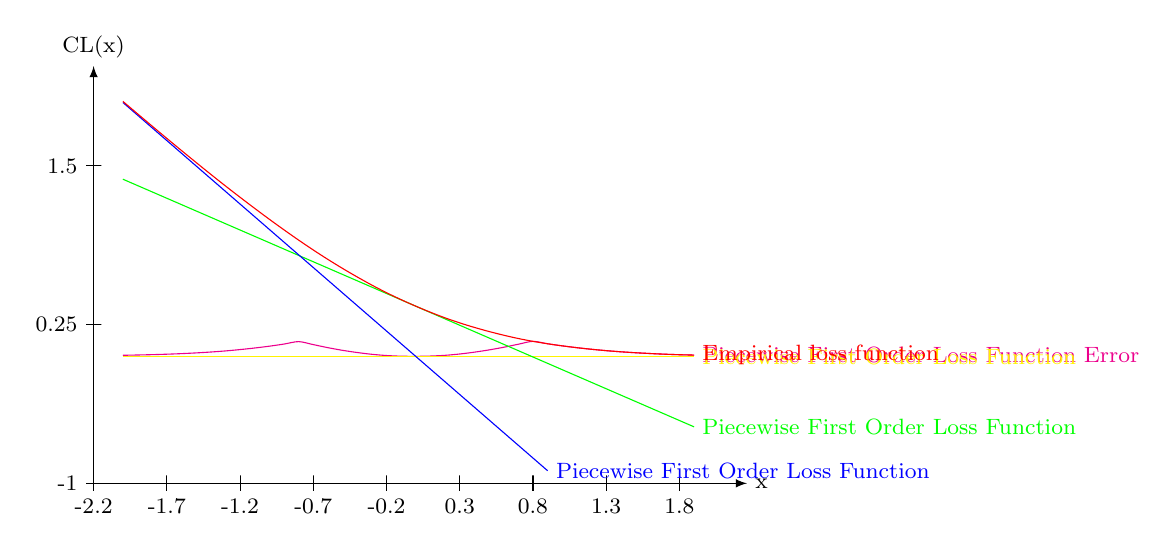
\begin{tikzpicture}[x=0.018604651162790697cm, y=0.016129032258064516cm]
\footnotesize
\draw [-latex] ([xshift=-0mm] 0.0,0) -- ([xshift=3mm] 430.00000000000006,0) node[right] {x};
\draw (0.0,0) -- +(0mm,1mm) -- +(0mm,-1mm) node[below] {-2.2};
\draw (50.0,0) -- +(0mm,1mm) -- +(0mm,-1mm) node[below] {-1.7};
\draw (100.0,0) -- +(0mm,1mm) -- +(0mm,-1mm) node[below] {-1.2};
\draw (150.0,0) -- +(0mm,1mm) -- +(0mm,-1mm) node[below] {-0.7};
\draw (200.0,0) -- +(0mm,1mm) -- +(0mm,-1mm) node[below] {-0.2};
\draw (250.0,0) -- +(0mm,1mm) -- +(0mm,-1mm) node[below] {0.3};
\draw (300.0,0) -- +(0mm,1mm) -- +(0mm,-1mm) node[below] {0.8};
\draw (350.0,0) -- +(0mm,1mm) -- +(0mm,-1mm) node[below] {1.3};
\draw (400.0,0) -- +(0mm,1mm) -- +(0mm,-1mm) node[below] {1.8};
\draw [-latex] ([yshift=-0mm] 0,0.0) -- ([yshift=3mm] 0, 310.0) node[above] {CL(x)};
\draw (0,0.0) -- +(1mm,0mm) -- +(-1mm,0mm) node[left] {-1};
\draw (0,125.0) -- +(1mm,0mm) -- +(-1mm,0mm) node[left] {0.25};
\draw (0,250.0) -- +(1mm,0mm) -- +(-1mm,0mm) node[left] {1.5};
\draw [smooth, color=magenta, mark= , style=solid] plot coordinates {%
(20.00,100.8324) %   (-2.000000,  0.008324)
(30.00,101.0702) %   (-1.900000,  0.010702)
(40.00,101.3396) %   (-1.800000,  0.013396)
(50.00,101.6962) %   (-1.700000,  0.016962)
(60.00,102.1470) %   (-1.600000,  0.021470)
(70.00,102.7161) %   (-1.500000,  0.027161)
(80.00,103.4140) %   (-1.400000,  0.034140)
(90.00,104.2668) %   (-1.300000,  0.042668)
(100.00,105.3393) %   (-1.200000,  0.053393)
(110.00,106.5764) %   (-1.100000,  0.065764)
(120.00,108.0063) %   (-1.000000,  0.080063)
(130.00,109.6786) %   (-0.900000,  0.096786)
(140.00,111.5993) %   (-0.800000,  0.115993)
(150.00,109.2472) %   (-0.700000,  0.092472)
(160.00,106.8324) %   (-0.600000,  0.068324)
(170.00,104.7378) %   (-0.500000,  0.047378)
(180.00,103.0197) %   (-0.400000,  0.030197)
(190.00,101.6150) %   (-0.300000,  0.016150)
(200.00,100.6510) %   (-0.200000,  0.006510)
(210.00,100.1281) %   (-0.100000,  0.001281)
(220.00,100.0059) %   (0.000000,  0.000059)
(230.00,100.2355) %   (0.100000,  0.002355)
(240.00,100.8168) %   (0.200000,  0.008168)
(250.00,101.8511) %   (0.300000,  0.018511)
(260.00,103.2972) %   (0.400000,  0.032972)
(270.00,105.0730) %   (0.500000,  0.050730)
(280.00,107.1586) %   (0.600000,  0.071586)
(290.00,109.5518) %   (0.700000,  0.095518)
(300.00,111.8170) %   (0.800000,  0.118170)
(310.00,109.9088) %   (0.900000,  0.099088)
(320.00,108.2629) %   (1.000000,  0.082629)
(330.00,106.8267) %   (1.100000,  0.068267)
(340.00,105.5723) %   (1.200000,  0.055723)
(350.00,104.4888) %   (1.300000,  0.044888)
(360.00,103.5889) %   (1.400000,  0.035889)
(370.00,102.8489) %   (1.500000,  0.028489)
(380.00,102.2247) %   (1.600000,  0.022247)
(390.00,101.6941) %   (1.700000,  0.016941)
(400.00,101.2882) %   (1.800000,  0.012882)
(410.00,100.9844)} %   (1.900000,  0.009844)
 node[right] {Piecewise First Order Loss Function Error};
\draw [smooth, color=yellow, mark= , style=solid] plot coordinates {%
(20.00,100.0000) %   (-2.000000,  0.000000)
(30.00,100.0000) %   (-1.900000,  0.000000)
(40.00,100.0000) %   (-1.800000,  0.000000)
(50.00,100.0000) %   (-1.700000,  0.000000)
(60.00,100.0000) %   (-1.600000,  0.000000)
(70.00,100.0000) %   (-1.500000,  0.000000)
(80.00,100.0000) %   (-1.400000,  0.000000)
(90.00,100.0000) %   (-1.300000,  0.000000)
(100.00,100.0000) %   (-1.200000,  0.000000)
(110.00,100.0000) %   (-1.100000,  0.000000)
(120.00,100.0000) %   (-1.000000,  0.000000)
(130.00,100.0000) %   (-0.900000,  0.000000)
(140.00,100.0000) %   (-0.800000,  0.000000)
(150.00,100.0000) %   (-0.700000,  0.000000)
(160.00,100.0000) %   (-0.600000,  0.000000)
(170.00,100.0000) %   (-0.500000,  0.000000)
(180.00,100.0000) %   (-0.400000,  0.000000)
(190.00,100.0000) %   (-0.300000,  0.000000)
(200.00,100.0000) %   (-0.200000,  0.000000)
(210.00,100.0000) %   (-0.100000,  0.000000)
(220.00,100.0000) %   (0.000000,  0.000000)
(230.00,100.0000) %   (0.100000,  0.000000)
(240.00,100.0000) %   (0.200000,  0.000000)
(250.00,100.0000) %   (0.300000,  0.000000)
(260.00,100.0000) %   (0.400000,  0.000000)
(270.00,100.0000) %   (0.500000,  0.000000)
(280.00,100.0000) %   (0.600000,  0.000000)
(290.00,100.0000) %   (0.700000,  0.000000)
(300.00,100.0000) %   (0.800000,  0.000000)
(310.00,100.0000) %   (0.900000,  0.000000)
(320.00,100.0000) %   (1.000000,  0.000000)
(330.00,100.0000) %   (1.100000,  0.000000)
(340.00,100.0000) %   (1.200000,  0.000000)
(350.00,100.0000) %   (1.300000,  0.000000)
(360.00,100.0000) %   (1.400000,  0.000000)
(370.00,100.0000) %   (1.500000,  0.000000)
(380.00,100.0000) %   (1.600000,  0.000000)
(390.00,100.0000) %   (1.700000,  0.000000)
(400.00,100.0000) %   (1.800000,  0.000000)
(410.00,100.0000)} %   (1.900000,  0.000000)
 node[right] {Piecewise First Order Loss Function};
\draw [smooth, color=green, mark= , style=solid] plot coordinates {%
(20.00,239.4891) %   (-2.000000,  1.394891)
(30.00,234.4891) %   (-1.900000,  1.344891)
(40.00,229.4891) %   (-1.800000,  1.294891)
(50.00,224.4891) %   (-1.700000,  1.244891)
(60.00,219.4891) %   (-1.600000,  1.194891)
(70.00,214.4891) %   (-1.500000,  1.144891)
(80.00,209.4891) %   (-1.400000,  1.094891)
(90.00,204.4891) %   (-1.300000,  1.044891)
(100.00,199.4891) %   (-1.200000,  0.994891)
(110.00,194.4891) %   (-1.100000,  0.944891)
(120.00,189.4891) %   (-1.000000,  0.894891)
(130.00,184.4891) %   (-0.900000,  0.844891)
(140.00,179.4891) %   (-0.800000,  0.794891)
(150.00,174.4891) %   (-0.700000,  0.744891)
(160.00,169.4891) %   (-0.600000,  0.694891)
(170.00,164.4891) %   (-0.500000,  0.644891)
(180.00,159.4891) %   (-0.400000,  0.594891)
(190.00,154.4891) %   (-0.300000,  0.544891)
(200.00,149.4891) %   (-0.200000,  0.494891)
(210.00,144.4891) %   (-0.100000,  0.444891)
(220.00,139.4891) %   (0.000000,  0.394891)
(230.00,134.4891) %   (0.100000,  0.344891)
(240.00,129.4891) %   (0.200000,  0.294891)
(250.00,124.4891) %   (0.300000,  0.244891)
(260.00,119.4891) %   (0.400000,  0.194891)
(270.00,114.4891) %   (0.500000,  0.144891)
(280.00,109.4891) %   (0.600000,  0.094891)
(290.00,104.4891) %   (0.700000,  0.044891)
(300.00,99.4891) %   (0.800000,  -0.005109)
(310.00,94.4891) %   (0.900000,  -0.055109)
(320.00,89.4891) %   (1.000000,  -0.105109)
(330.00,84.4891) %   (1.100000,  -0.155109)
(340.00,79.4891) %   (1.200000,  -0.205109)
(350.00,74.4891) %   (1.300000,  -0.255109)
(360.00,69.4891) %   (1.400000,  -0.305109)
(370.00,64.4891) %   (1.500000,  -0.355109)
(380.00,59.4891) %   (1.600000,  -0.405109)
(390.00,54.4891) %   (1.700000,  -0.455109)
(400.00,49.4891) %   (1.800000,  -0.505109)
(410.00,44.4891)} %   (1.900000,  -0.555109)
 node[right] {Piecewise First Order Loss Function};
\draw [smooth, color=blue, mark= , style=solid] plot coordinates {%
(20.00,299.9372) %   (-2.000000,  1.999372)
(30.00,289.9372) %   (-1.900000,  1.899372)
(40.00,279.9372) %   (-1.800000,  1.799372)
(50.00,269.9372) %   (-1.700000,  1.699372)
(60.00,259.9372) %   (-1.600000,  1.599372)
(70.00,249.9372) %   (-1.500000,  1.499372)
(80.00,239.9372) %   (-1.400000,  1.399372)
(90.00,229.9372) %   (-1.300000,  1.299372)
(100.00,219.9372) %   (-1.200000,  1.199372)
(110.00,209.9372) %   (-1.100000,  1.099372)
(120.00,199.9372) %   (-1.000000,  0.999372)
(130.00,189.9372) %   (-0.900000,  0.899372)
(140.00,179.9372) %   (-0.800000,  0.799372)
(150.00,169.9372) %   (-0.700000,  0.699372)
(160.00,159.9372) %   (-0.600000,  0.599372)
(170.00,149.9372) %   (-0.500000,  0.499372)
(180.00,139.9372) %   (-0.400000,  0.399372)
(190.00,129.9372) %   (-0.300000,  0.299372)
(200.00,119.9372) %   (-0.200000,  0.199372)
(210.00,109.9372) %   (-0.100000,  0.099372)
(220.00,99.9372) %   (0.000000,  -0.000628)
(230.00,89.9372) %   (0.100000,  -0.100628)
(240.00,79.9372) %   (0.200000,  -0.200628)
(250.00,69.9372) %   (0.300000,  -0.300628)
(260.00,59.9372) %   (0.400000,  -0.400628)
(270.00,49.9372) %   (0.500000,  -0.500628)
(280.00,39.9372) %   (0.600000,  -0.600628)
(290.00,29.9372) %   (0.700000,  -0.700628)
(300.00,19.9372) %   (0.800000,  -0.800628)
(310.00,9.9372)} %   (0.900000,  -0.900628)
 node[right] {Piecewise First Order Loss Function};
\draw [smooth, color=red, mark= , style=solid] plot coordinates {%
(20.00,300.7696) %   (-2.000000,  2.007696)
(30.00,291.0074) %   (-1.900000,  1.910074)
(40.00,281.2768) %   (-1.800000,  1.812768)
(50.00,271.6333) %   (-1.700000,  1.716333)
(60.00,262.0842) %   (-1.600000,  1.620842)
(70.00,252.6533) %   (-1.500000,  1.526533)
(80.00,243.3512) %   (-1.400000,  1.433512)
(90.00,234.2040) %   (-1.300000,  1.342040)
(100.00,225.2765) %   (-1.200000,  1.252765)
(110.00,216.5136) %   (-1.100000,  1.165136)
(120.00,207.9435) %   (-1.000000,  1.079435)
(130.00,199.6158) %   (-0.900000,  0.996158)
(140.00,191.5365) %   (-0.800000,  0.915365)
(150.00,183.7362) %   (-0.700000,  0.837362)
(160.00,176.3214) %   (-0.600000,  0.763214)
(170.00,169.2268) %   (-0.500000,  0.692268)
(180.00,162.5087) %   (-0.400000,  0.625087)
(190.00,156.1040) %   (-0.300000,  0.561040)
(200.00,150.1401) %   (-0.200000,  0.501401)
(210.00,144.6171) %   (-0.100000,  0.446171)
(220.00,139.4950) %   (0.000000,  0.394950)
(230.00,134.7246) %   (0.100000,  0.347246)
(240.00,130.3058) %   (0.200000,  0.303058)
(250.00,126.3401) %   (0.300000,  0.263401)
(260.00,122.7863) %   (0.400000,  0.227863)
(270.00,119.5620) %   (0.500000,  0.195620)
(280.00,116.6477) %   (0.600000,  0.166477)
(290.00,114.0409) %   (0.700000,  0.140409)
(300.00,111.8170) %   (0.800000,  0.118170)
(310.00,109.9088) %   (0.900000,  0.099088)
(320.00,108.2629) %   (1.000000,  0.082629)
(330.00,106.8267) %   (1.100000,  0.068267)
(340.00,105.5723) %   (1.200000,  0.055723)
(350.00,104.4888) %   (1.300000,  0.044888)
(360.00,103.5889) %   (1.400000,  0.035889)
(370.00,102.8489) %   (1.500000,  0.028489)
(380.00,102.2247) %   (1.600000,  0.022247)
(390.00,101.6941) %   (1.700000,  0.016941)
(400.00,101.2882) %   (1.800000,  0.012882)
(410.00,100.9844)} %   (1.900000,  0.009844)
 node[right] {Empirical loss function};
\end{tikzpicture}
\end{center}
\caption{Piecewise linearization}
\end{figure}
\end{document}
